\documentclass[../main]{subfiles}
\begin{document}

\chapter{相关文献的研究现状}%
\label{cha:相关文献的研究现状}

\section{基于定标的非均匀性校正}%
\label{sec:基于定标的非均匀性校正}

在考虑硬件实时性时,定标的非均匀性校正是目前已经适用化的技术。但需要对系统进行周
期性的重复定标以消除参数漂移的影响,这就相应地增加了系统的复杂性,降低了系统的可
靠性和响应速度;对于机载、弹载探测器不易做到快速反应。

基于定标的非均匀性校正算法如图\ref{fig:增益校正和偏移校正}和图\ref{fig:分段校正}
所示。

\begin{figure}[htbp]
	\centering
	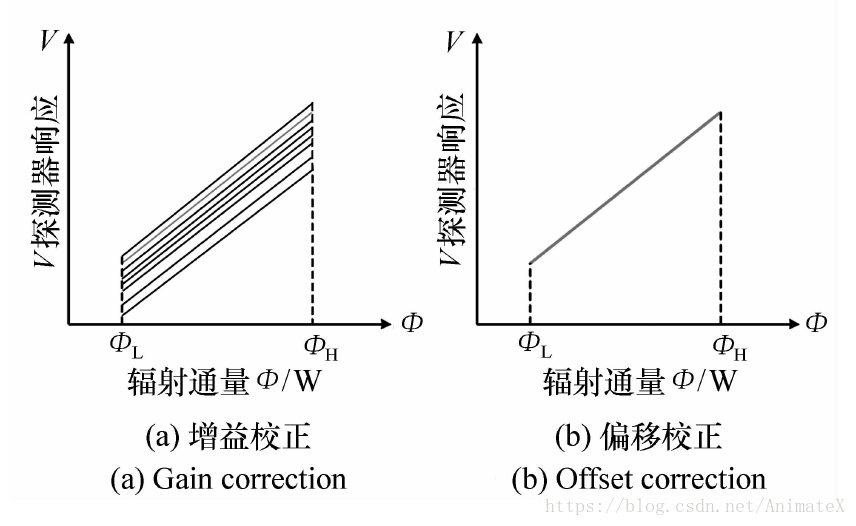
\includegraphics[width=0.8\linewidth]{compare.png}
	\caption{增益校正和偏移校正}
	\label{fig:增益校正和偏移校正}
\end{figure}

\begin{figure}[htbp]
	\centering
	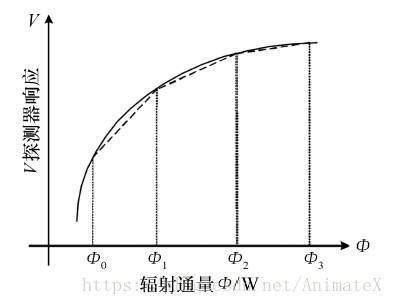
\includegraphics[width=0.6\linewidth]{section.png}
	\caption{分段校正}
	\label{fig:分段校正}
\end{figure}

基于标定技术的算法无法永久适用于各像元的差别性漂移,从而使得我们长时间使用时必须
进行标定。这在实际使用中带来很大不便,自适应非均匀性校正方法是非均匀性校正发展的
必然趋势。

\section{基于场景的非均匀性校正}%
\label{sec:基于场景的非均匀性校正}

基于场景的校正算法不但省略了参考辐射源,使系统处理流程得到简化,提高系统的稳定性
,而且可以有效地消除参数特性漂移的影响,实现高精度、大动态范围的自适应非均匀校正
。基于场景的非均匀性校正不需要红外参照源\footnote{基于定标的非均匀性校正需要黑体
定标},从实际场景提取校正参数,实现系统简洁,克服了器件的空间非均匀性影响和周期
性定标问题 ,具有自适应校正的优点。也正是基于这些优点,基于场景的校正方法近年来
出现了许多新的研究成果 ,成为红外成像技术和红外成像电子学处理方法的研究热点。

自从基于场景校正这一概念出现以来,国外学者便给予了高度关注,并取得了大量的研究成
果与一批良好的校正算法。总的来说,这些算法都是通过两大类途径实现的。

\begin{enumerate}

	\item 一类是基于 \emph{统计}的,基于统计类的技术通常对于焦平面每个像元接
		收到的辐射量作一些时间上或者空间上的统计假设,在此假设的基础上不
		断修正校正参数,校正焦平面的非均匀性。其中最具代表性的技术有时域
		高通法,统计恒定法,神经网络法,恒定范围法及其的相应的扩展形式,
		如统计维纳滤波法,卡尔曼滤波法等。该类算法一般要求目标场景与
		IRFPA 器件相对运动以使IRFPA器件中所有探测单元在一段时间内所接收
		到的目标场景辐射的满足一定的统计假设。然而,由于图像场景的多样性
		,该假设不一定能够得到满足,因此这类校正算法经常伴随较为严重的鬼
		影问题。

	\item 另一类是基于 \emph{配准}的,这类技术认为,在较短的时间间隔内,若观
		察场景中相同的位置时,每个像元的响应也应该是相同的,因此这类技术
		需要准确的估计帧与帧之间的移动。如图\ref{fig:相邻两帧图像}所示
		。其中比较有代表性的技术有全景图积累法,代数校正法等。但是这类算
		法由于其要求限制较多,计算量与存储量较大,且校正误差易逐级累计传
		播,所以较难达到实用。

\end{enumerate}

\begin{figure}[htbp]
\centering
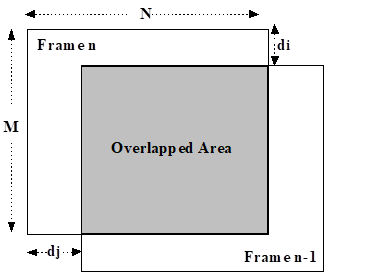
\includegraphics[width=0.6\linewidth]{frame.png}
\caption{相邻两帧图像}
\label{fig:相邻两帧图像}
\end{figure}

\subsection{神经网络法}%
\label{sub:神经网络法}

如图\ref{fig:传统的神经网络用4邻域均值代替真实值},传统的基于BP神经网络的非均匀
性校正算法用4邻域均值代替真实值。当目标不动后突然运动容易出现鬼影。而且存在期望
值不准确、误差函数精度不高和学习速度不适应网络变化的缺点。

\begin{figure}[htbp]
	\centering
	\includegraphics[width=0.4\linewidth]{5.pdf}
	\caption{传统的神经网络用4邻域均值代替真实值}
	\label{fig:传统的神经网络用4邻域均值代替真实值}
\end{figure}

传统的神经网络由于采用了四邻域均值代替期望值,使得图像呈现低通的特性。樊秀梅
\cite{樊秀梅2010基于}将加权中值滤波处理后的结果作为期望输出,并在神经网络算法中
权值修正时加入了动量项,加快了算法的收敛速度。

郑德忠\cite{郑德忠2010应用于非均匀性校正的改进的神经网络算法}将目标像元与其4邻近
像元的像素值进行比较,按偏差值的大小进行排序,再增加权系数来计算期望值。又分析了
神经网络出现的局部极小问题,在原有的误差函数基础上引入了隐层饱和度的计算式;并提
出了根据总误差值之比来调节学习速度。

\cite{Torres2003Adaptive}在没有对原始数据中呈现的非均匀性的种类或数量做出任何假
设的情况下,采用神经网络方法进行非均匀性补偿。因此该方法的强度和鲁棒性依赖于通过
在参数估计学习过程中使用优化技术来避免重影伪影的存在。

\begin{figure}[htbp]
\centering
\includegraphics[width=0.8\linewidth]{BP.pdf}
\caption{神经网络}
\label{fig:神经网络}
\end{figure}

赖睿\cite{赖睿2009场景自适应的红外焦平面阵列非均匀性校正新方法}重新设计了隐藏层
的结构,有助于更准确地估计出目标的期望值。此外,将基于变步长归一化的自适应滤波技
术引入到校正参数估计过程中,具有较快的收敛速度和较高的稳定性。

\subsection{时域高通法}%
\label{sub:时域高通法}

时域高通滤波法只能校正偏置的缓慢漂移,对增益的漂移没有办法;且为了滤除低频,要求
场景一直运动。否则一样容易出现鬼影。

早在1997年,Scribner 就在\cite{Scribner1990Nonuniformity, Scribner1991Adaptive}
总结了时间高通法和神经网络法的优点,指出两者与生物视网膜处理有相似之处。并与传统
的非均匀性校正技术进行了比较。预言自适应技术在未来的红外焦平面传感器中将非常有用
,因为它们能够在无校准源的情况下适应大范围的背景流量,同时也可以在大多数工作条件
下提供更高的灵敏度。

刘缠牢\cite{刘缠牢2006红外图像非均匀性校正高通滤波算法的改进}为了调节系统的截止
频率,在时域高通滤波法中增加了一个调节因子,目的是选择合适的调节因子能够尽可能
校正焦平面阵列的非均匀性,改进其校正效果。

Sanmartin\cite{Sanmartin2008Extended}在估计时间窗足够短的假设下,偏移量就可以看
作是噪声中的一个常数。提出了一种递归滤波器来估计红外成像系统中存在的探测器偏移非
均匀性噪声。由于偏移量是非平稳的,当新的红外成像数据块到达时,必须计算偏移量
的新估计。

Martin\cite{Martin2010Block} 在Sanmartin\cite{Sanmartin2008Extended}的基础上,放
宽了对偏移噪声平稳性的限制,利用Gauss-Markov随机过程描述了偏移的动力学特性,推导
了一种利用红外数据块估计偏移量的递归滤波器。

\subsection{统计恒定法}%
\label{sub:统计恒定法}

在基于红外焦平面阵列相机的非均匀校正方法中,统计方法由于计算复杂度低而得到了很好
的研究。然而,当违反统计算法的假设时,它们的性能很差此外,许多技术,如全局常数统
计方法,通常需要数万个图像帧才能获得良好的结果。

Hardie\cite{Hardie2000Scene}使用了总方差法,虽然该方法在现在不再有新意,但因
其经典性仍被广泛引用。

Harris\cite{Harris1999Nonuniformity}和Pezoa\cite{Pezoa2004An}总结了常数统计法。

Strojnik\cite{Strojnik1997Nonuniformity}在增益和偏移量的变化是平滑的简单假设下,
提供了使用数字实现的一维和二维图像的常数统计法校准结果。证明了在收敛速度和计算复
杂度上,常数统计法优于现有的基于最小均方的
Scribner\cite{Scribner1990Nonuniformity, Scribner1991Adaptive} 非均匀性校正算法
。

文献\cite{何大竺2000应用常值统计约束的非均匀性校正——模拟与数字实现}与文献
\cite{Strojnik1997Nonuniformity}相似度很高。可能是参照了文献
\cite{Strojnik1997Nonuniformity}

Hardie\cite{Hardie2009Scene}改进了Scribner\cite{Scribner1990Nonuniformity,
Scribner1991Adaptive}的非均匀性校正算法。通过在更新一种新的选通操作,在缺少时间
变化时停止更新来显著减少由算法产生的重影伪影。

Zuo\cite{Zuo2011Scene}静态地认为时间常数分布的空间尺度随时间而扩展,于是,在假设
非均匀性分布在较高的空间频率域的前提下,提出了偏多尺度常数统计法。在估计的空间范
围逐渐扩大时能保证非均匀性的快速补偿。该方法的优点在于其简单、计算复杂度低以及收
敛速度和校正精度之间的良好折衷。

\subsection{Wiener滤波}%
\label{sub:Wiener滤波}

Hou\cite{Hou2010Image}基于均匀检测器的假设,提出了基于卷积的退化模型,通过一种基
于改进维纳滤波器的退化恢复方法--牛顿-拉斐逊法搜索优化参数。在实际应用中不能满
足假设。因此需要对非均匀性进行盲像素补偿等预处理以满足假设。

\subsection{Kalman滤波法}%
\label{sub:Kalman滤波法}

Torres\cite{Torres2003Scene}在给定的帧序列内,假定焦平面阵列中每个探测器的增益和
偏压为常数,但允许它们在一定的时间和工作条件们随离散时间高斯 -马尔可夫过程从一个
序列随机漂移到另一个序列。基于Kalman滤波器的逆协方差形式,估计焦平面阵列中每个探
测器的增益和偏差,并在它们随时间漂移时对它们进行最佳更新

Pezoa\cite{Pezoa2006Multimodel}并行使用一组卡尔曼滤波器,提出了一种对场景和传感
器特性的变化和不确定性都具有鲁棒性的方法。每个滤波器根据自己的动态模型参数,独立
地估计包含传感器的增益和偏置矩阵的状态变量。然后,算法的监督部分通过形成由每个卡
尔曼滤波器给出的所有估计的加权叠加来生成状态变量的最终估计。根据后验似然原理,迭
代计算和更新权重。

Torres\cite{Torres2003Kalman}依赖于数据中的一定时空多样性条件,提出的一种在传感
器工作条件随时间变化时捕获固定模式噪声中缓慢随机漂移的Gauss-Markov框架。在每个探
测器的增益和偏置的时间随机模型下,推导了一个卡尔曼滤波器,提出了一种基于场景数据
的红外焦平面阵列传感器增益和偏置非均匀性自适应估计的统计方法。

\subsection{代数校正算法}%
\label{sub:代数校正算法}

基于统计的校正算法要求探测器像元的响应独立同分布,线性响应;对场景的要求是场景必
须一直运动,且运动幅度较大;而静止后突然运动非常容易出现鬼影。基于 \emph{配准}
的算法可避免这个问题。其中代数校正算法是最早的研究方向。

Hayat\cite{Hayat1999Statistical}针对焦平面阵列红外成像系统响应中空间非均匀性和时
间裂缝引起的固定模式噪声,提出了一种统计补偿算法--Hayat统计法。该算法利用初始
场景数据对每个探测器单元的增益、偏移量和加性电子噪声方差进行初始估计然后,该算法
利用后续帧更新这些参数,并利用更新后的参数通过上均方误差有限脉冲响应滤波器恢复真
实图像。

Liu\cite{Liu2011Non}提出了一种基于运动可控微扫描平台和周界光阑条的红外焦平面非均
匀性校正算法。首先对周长检测器进行一点标定,然后基于相邻帧的可控运动,提出了一种
特殊的代数算法,将周长检测器的标定传递到未经校正的帧内这样,就可以计算出整个视场
的偏压参数。该算法可以方便地与亚像素成像相结合,从而提高热成像系统的质量(图像的
空间分辨率和均匀性)。

Ratliff\cite{Ratliff2002An}提出了一种基于场景的焦平面阵列非均匀性补偿算法。基于图像序列
中帧间亚像素位移的估计,结合运动的线性插值模型,从代数上提取关于偏移非均匀性的信
息。

\subsection{全景图积累法}%
\label{sub:全景图积累法}

Wenyi\cite{Wenyi2008Scene}提出了一种新的基于配准的非均匀性校正超分辨率方法。该方
法由基于统计场景的非均匀性校正方法引导。利用一个综合的成像模型和精确的参数运动估
计,能够消除严重的非均匀性和亚像素运动,同时提高图像的分辨率。

Tendero\cite{Tendero2012Non}提出了一种有效的基于自适应灰度调整的单幅图像条纹噪声
去除方法。从每个帧中提取所有的条纹噪声谱,然后通过亚像素配准剔除相对平稳的图像,
得到连续运动的图像序列。通过积累图像序列的相同频谱,我们可以获得准确的条纹噪声。
单帧去条纹的效果还不错。

Thurman\cite{ThurmanEfficient}比较了三种新的基于非线性优化和矩阵乘离散傅里叶变换
的二维平移图像配准算法的平移不变误差度量。这些算法可以在很小的计算时间内实现与传
统快速傅里叶变换上采样方法相当的精度,并且大大降低了内存需求。

\section{其它算法}%
\label{sec:其它算法}

Godoy\cite{Godoy2008Noise}基于这样一个假设,即与加性空间固定模式噪声相关的噪声源
可用于红外相机。在非极端情况下该假设基本成立。据此,他提出了噪声抵消法--一种基
于噪声抵消的加性补偿算法。该算法的一个重要特点是所有的计算都简化为一个简单的方程
,从而可以对原始图像进行偏差补偿。利用该方法对利用实际红外图像序列对算法性能进行
了测试,并与一些经典方法进行了比较。

Nie\cite{Nie2010Infrared}根据盲信息源分解技术,将红外图像分为信号源和噪声源,提
出了一种基于快速独立分量盲分离的非均匀性校正方法。通过对真实红外图像的线性校正算
法和常数统计法的实验对比分析,该算法不仅抑制了基于物理校正源的线性校正算法的系统
响应漂移和环境温度变化的影响,也部分克服了基于场景的非均匀性校正在统计样本和尺
寸方面的不足。

Esteban\cite{Esteban2011Total} 基于估计辐照度总变化的最小化,并利用交替最小化策
略,采用各向同性总变化方法对得到的函数进行优化。在应用于不同的真实红外图像集时,
该方法不仅能以较快的收敛速度准确估计焦平面阵列中每个探测器的非均匀参数,而且能形
成较少的重影伪影。

Yong\cite{Yong2009Scene}采用帧间预测方法对真实场景进行估计阵列传感器的增益和偏置
非均匀性。通过直线拟合技术,利用估计的场景和探测器获得的相应观测数据来更新增益和
偏差。利用这些非均匀性参数,通过计算一个非常简单的公式得到每个探测器的补偿输出。
该算法的优点在于其计算复杂度和存储要求以及捕获非均匀性参数中的时间漂移的能力。

如图\ref{fig:基于帧间配准误差最小化的非均匀性校正的原理图}所示,Chao
\cite{Chao2011Scene} 提出了一种基于帧间配准的红外焦平面阵列非均匀性校正方法该方
法通过估计两个相邻帧之间的全局平移,并将两幅正确注册的图像之间的均方误差最小化,
使同一场景的任意两个检测器产生相同的输出值。这样就避免了配准误差的积累,实现了非
均匀性校正。

\begin{figure}[htbp]
\centering
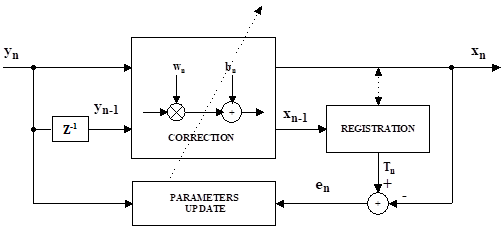
\includegraphics[width=0.8\linewidth]{calibrate.png}
\caption{基于帧间配准误差最小化的非均匀性校正的原理图}
\label{fig:基于帧间配准误差最小化的非均匀性校正的原理图}
\end{figure}

除此之外另有学者提出了综合利用多种经典算法的新算法。

时域高通滤波法简单,易于实现的优点让其仍有用武之地。在既有加性噪声又有乘性噪声时
校正效果不佳。神经元网络算法在噪声较强时,校正效果受到了限制 。针对既有加性噪声
,又有乘性噪声,且加性噪声较强的情况,仿真证明红外焦平面非均匀校正的综合处理算法
具有较好的校正效果。\cite{张小军2003红外焦平面非均匀校正的综合处理算法}

\section{评价方法}%
\label{sec:评价方法}

校正算法众多导致如何评价算法的优劣也成为了值得研究的方向。

汪民\cite{汪民2007基于校正率的红外焦平面阵列非均匀性校正评估新方法}提出一种新的
能对非均匀性校正效果进行定量计算的评估测度“校正率”。校正率以时域噪声为参考标准来
衡量图像非均匀特性,不仅可以反映图像显示效果,还可以反映图像测温精度.

Raz\cite{Raz2011A}指出一个有效的基于场景的非均匀性校正算法必须考虑时间和空间的限
制。他利用空间频域表示将图像中的距离自然转换为不同的空间频率,提供了研究基于场景
的非均匀性校正的时空关系的一个有效视角,证明了一种通过递归时间滤波器来实现这种校
正的方法,它将空间频率依赖性融入到校正速度中,使得在校正过程中可以很容易地设计出
时空关系利用多个特征成像运动模型,我们分析了运动对时空关系的影响,并演示了如何为
每个运动模型设计最佳的基于场景的非均匀性校正过程。

Martin\cite{Martin2007An}提出了有效粗糙度指数--一种与视觉评价结果一致的非均匀
性校正方法的性能指标。

Schulz\cite{Schulz1995Nonuniformity} 考虑了信号响应的非线性,利用多个辐射源和最
小二乘拟合逼近单个像素响应特性,定义了一个校正性能指标,用于估计校正后的剩余固定
模式噪声。

\end{document}

